\chapter{Large-Scale Toxicity Analysis} \label{large-scale-analysis}
Having chosen the detoxify unbiased model, we now use a large-scale pipeline to assign seven toxicity values between 0 and 1 to each toot for further analysis. Afterwards we compare the average toxicity levels on the instances with the moderation policies and instance rules to find out if there is a correlation between toxicity and moderation.

\section{Large-Scale Pipeline}
The pipeline is built using the Ray framework \cite{moritz:2018}, which enables distributed computing for efficient large-scale data processing. The pipeline consists of several stages: data reading, deduplication, toxicity prediction, and merging (Figure~\ref{fig:pipeline}).

\paragraph{Prerequisites}
The Ray environment is configured with specific settings for parallelism, memory, and number of cpu's per task to ensure efficient processing of large datasets. We run the tasks seperatly in parallel pipelines to avoid memory conflicts and cache our results between the stages. The pipeline is designed to run on a cluster with 507 CPU cores, 976GB of RAM, and 290GB of object store memory, by using 0.01 CPU cores per task, with a maximum of 100 tasks running in parallel. To ensure robustness, the pipeline is configured to retry failed tasks up to 10 times, with retry exceptions enabled to handle briefly flashing errors well.

These settings ensure that the pipeline can handle large datasets efficiently on our cluster while minimizing resource conflicts. The key to this scalability lies in our use of Ray's \textit{map\_batches}\footnote{url{https://docs.ray.io/en/latest/data/api/doc/ray.data.Dataset.map\_batches.html}} function combined with pandas\footnote{\url{https://pandas.pydata.org/docs/user\_guide/index.html}} DataFrames. The \texttt{map\_batches} operation processes data in manageable chunks, distributing the workload across available cluster resources. Each batch is converted to a pandas DataFrame, enabling us to utilise pandas' rich ecosystem of vectorized operations and transformations on each subset of data. This combination provides both horizontal scalability through Ray's distributed computing framework and vertical efficiency through pandas' optimized in-memory operations. The result is an elegant solution for designing complex parallel pipelines while maintaining the simplicity of working with familiar pandas operations.

\paragraph{Reading Toots from elasticsearch}\label{step:reading}
The pipeline's first stage retrieves Mastodon data from Elasticsearch using the following filters:

\begin{enumerate}
    \item \textbf{Temporal scope}: Only toots posted during 2024
    \item \textbf{Instance selection}: From 1,000 fully crawled instances
    \item \textbf{Content filters}:
    \begin{itemize}
        \item Original toots only (excluding reblogs/boosts)
        \item Text-only content (removing toots with media attachments)
        \item English-language labeled content
    \end{itemize}
\end{enumerate}

We use the \textit{ray\_elasticsearch}\footnote{\url{https://github.com/janheinrichmerker/ray-elasticsearch}} library for efficient Elasticsearch queries. The retrieved data contains the fields described in Table~\ref{dataset-fields}, including toot identifiers, content, instance information, and metadata flags. To avoid overloading the Elasticsearch cluster, we read data directly into local storage using the Parquet\footnote{\url{https://github.com/apache/parquet-java}} file format for efficient storage.

\paragraph{Language Detection using FastText}
Because the language labels given from Mastodon are just about the users main language, there are still non english toots in our dataset. The detoxify unbiased model is just trained for english toxicity detection. To ensure only English texts are processed, a language detection step is performed later on the deduplicated dataset. Therefore we use the FastText\footnote{\url{https://huggingface.co/facebook/fasttext-language-identification}} model to predict each toot’s language. We keep only those labeled as English for further analysis, thereby reducing the dataset by 3 million toots and 205 instances.
FastText is ideal for this task due to its use of subword information (character n-grams), which enables robust handling of informal language, misspellings, and slang common in social media texts. Its efficiency and accuracy in language detection ensure reliable filtering, even for short or noisy inputs \cite{joulin:2016}.

\begin{figure}[tb]
    \centering
    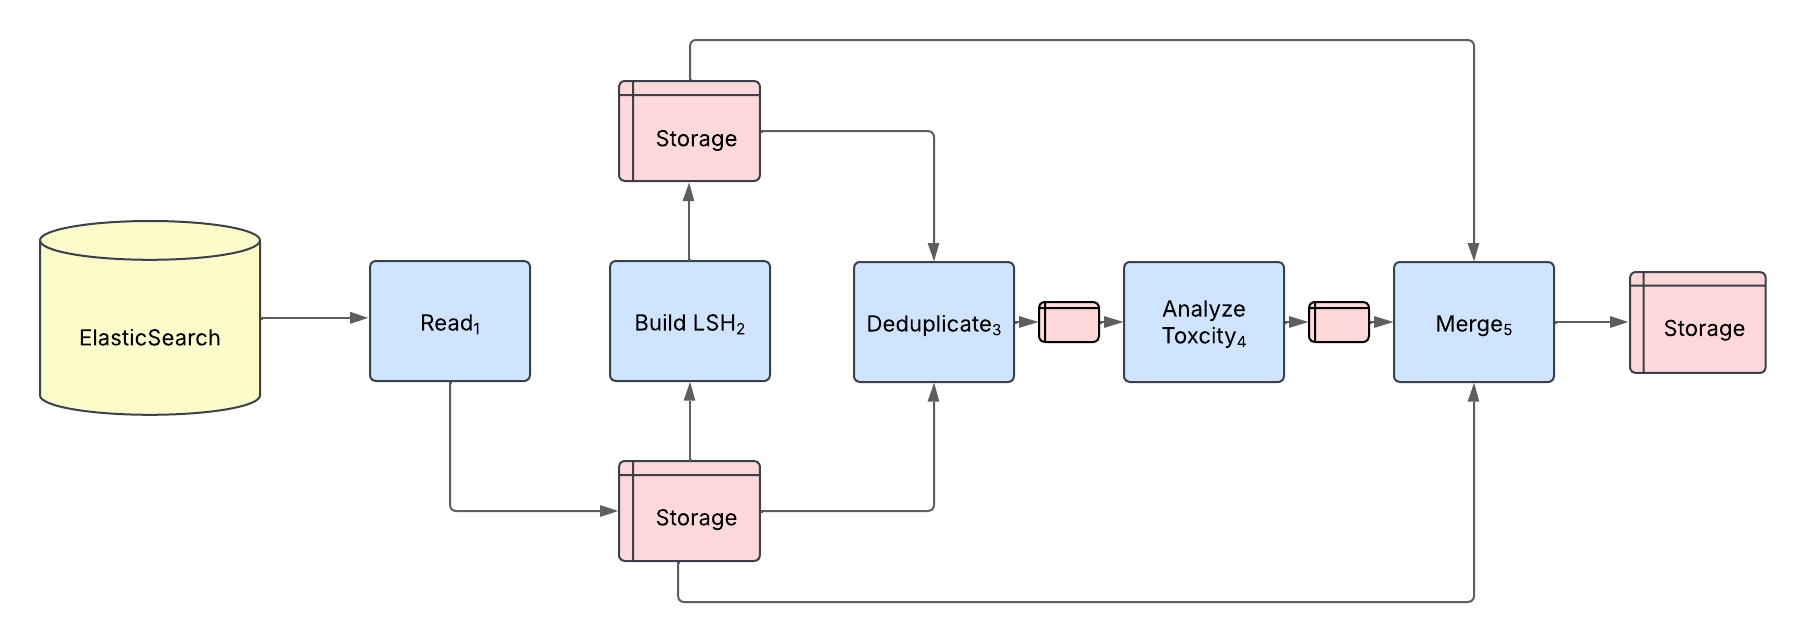
\includegraphics[width=\textwidth]{../material/pipeline.png}
    \caption{Data processing pipeline: 
    (\hyperref[step:reading]{1}) \textbf{Read \& Preprocess}: Reading data from the ElasticSearch database, extracting plaintext and calculating MinHash, then storing results; 
    (\hyperref[step:lsh]{2}) \textbf{Build LSH}: Building LSH index from processed data and storing it; 
    (\hyperref[step:dedup]{3}) \textbf{Deduplicate}: Near-duplicates are removed from processed data using the LSH index; 
    (\hyperref[step:toxicity]{4}) \textbf{Analyze Toxicity}: Performing toxicity analysis on deduplicated data; 
    (\hyperref[step:merge]{5}) \textbf{Merge}: Merging analyzed data with the original dataset using the LSH index. 
    Blue boxes represent processes, red indicates storage components, and yellow marks the external database.}
    \label{fig:pipeline}
\end{figure}

\subsection{Handling Large Datasets by Minhashbased Deduplication and Merging}
Because of the high duplication rate of 95\% in the original dataset, we planned to deduplicate the data before analyzing it. After the analysis by our model we wanted to merge the results back into the original dataset. The deduplication and merging processes are based on MinHash signatures, which allow us to efficiently identify near-duplicate toots without having to compare every toot against each other in the dataset. In our actual analysis on the 1\% subset we directly analyzed the toots without deduplication and merging, because the subset contains less than 50\% duplicates and without the deduplication and merging our analysis was much faster. But nethertheless we will explain the process here for future work.

\paragraph{Preperation for minhash-based Deduplication and Merging} 
Before we calculate the MinHash of every toot, we need to extract plaintext from the HTML content using the \textit{extract\_plain\_text} function from resiliparse \cite{bevendorff:2018}. On the plaintext we can simply calculate the MinHash using the datasketch API\footnote{\url{https://ekzhu.com/datasketch/documentation.html\#minhash}}. The MinHash provides an efficient way to estimate the Jaccard similarity between documents. The Jaccard similarity $J(A,B)$ between two sets $A$ and $B$ is defined as:

\begin{equation}
J(A,B) = \frac{|A \cap B|}{|A \cup B|}
\end{equation}

MinHash works by computing multiple hash values for each document's shingles (contiguous subsequences of words) and keeping only the minimum hash value for each permutation. The probability that the minimum hash values match for two toots equals their Jaccard similarity \cite{broder:2000}. Our implementation uses 64 permutations to balance storage requirements with similarity estimation accuracy.

\subsubsection{LSH Index Construction}\label{step:lsh} 
The deduplication and merging employ Locality-Sensitive Hashing (LSH) \cite{leskovec:2014} techniques to efficiently identify and remove near-duplicate toots from the dataset. The idea of LSH is to group similar toots into buckets through a process called banding. This approach works by dividing each document's MinHash signature into $b$ bands of $r$ rows each. For a document with a MinHash signature of length $n$, we ensure $b \times r \le n$. Each band is then processed separately through a hash function, and toots sharing identical hash values in any band are considered potential duplicates. By setting the jaccard similarity threshold to 0.9, the optimizer finds values for $b$ and $r$ so that the probability of two toots sharing a band is very high when their Jaccard similarity is $\geq90\%$. The threshold is chosen to 0.9 because jaccard similarity is just indicating word similarity but not semantic similarity. Because we don't want to remove toots that are just similar in words but not in meaning, we choose a much higher threshold than the maybe more realistic threshold of 0.58 explored by \citet{wu:2020} for similarity in short texts. 

We built one LSH index for the entire dataset. If this index gets queried, the response are all toot id's matching a jaccard similarity $\geq90\%$ to the queried toot.

\paragraph{MinHash-based Similarity Deduplication}\label{step:dedup} 
For each toot we query the LSH index by inserting one toot's minhash and receving all similar ids in the same bucket. Within each group of near-duplicates, we retain only the toot with the smallest id value, ensuring deterministic selection while removing duplicates. This approach guarantees that only one representative instance of each near-duplicate group remains in the final dataset.

\paragraph{MinHash-based Similarity Merging}\label{step:merge}
The LSH index is queried for each toot in our subset to find similar toots. Because we kept the smallest id in the deduplication, now the smallest id in the query results always matches an id in the deduplicated dataset. We concatenate the matched analyzed toot from the deduplicated dataset with the original toot we used for our query. The toots now containing all relevant information and the the dataset for further analysis is created.

\section{Toxicity Analysis}\label{step:toxicity}
We use the detoxify unbiased model to perform zero-shot toxicity prediction on the 1\% subset. Zero-shot prediction means the model was not fine-tuned on Mastodon toots and makes predictions using only its pretrained knowledge. For each toot, the model predicts scores for all seven toxicity categories defined in Table~\ref{toxicity-categories}.

\begin{figure}[tb]
    \centering
    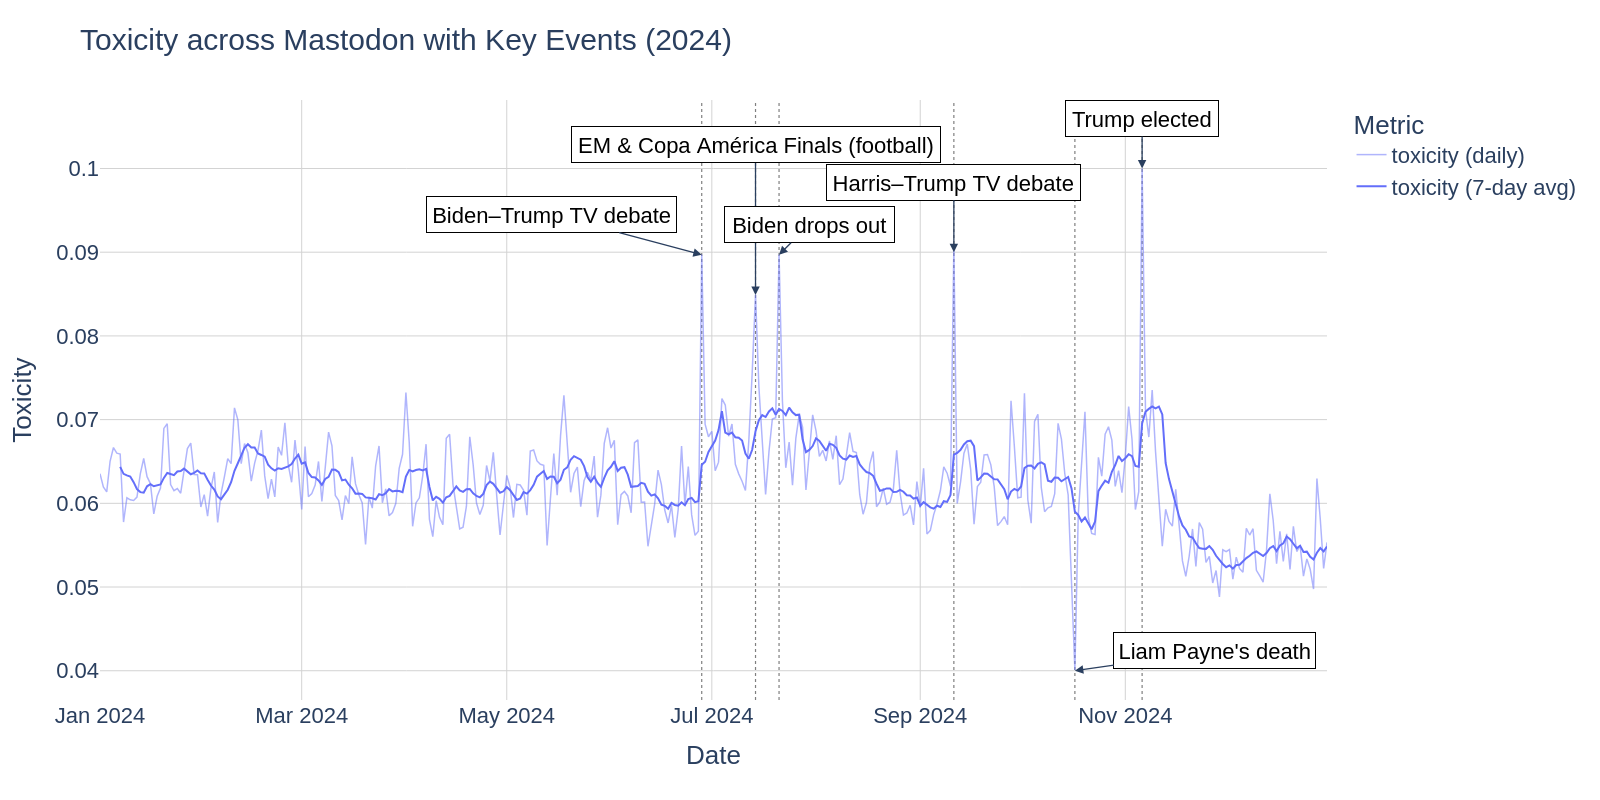
\includegraphics[width=\textwidth]{../material/toxicity_2024.png}
    \caption{Distribution of the daily mean value and a 7-day average for the toxicity category over the year~2024. The main peaks are marked with events that occurred on that day, which may have influenced the toxicity value.}
    \label{toxicity-2024}
\end{figure}

\paragraph{Peak analysis of Toxicity timeline} 
Figure~\ref{toxicity-2024} shows the distribution of the daily mean value and a 7-day average for the toxicity category over the year~2024. Several peaks occur during major events, influencing the toxicity value. Overall, the toxicity value remains stable between 0.06 and 0.07 but drops toward the end of the year to 0.05. This drop may be explained by the increase in the total number of toots (Figure~\ref{toot-distribution}), indicating that toxic communities did not grow as much as non-toxic ones.

The most prominent peak coincides with the U.S.\ election results on November~6, 2024, when Donald Trump was elected president. The only significant negative peak occurs on October~17, one day after Liam Payne's death. This peak likely results from a sudden increase in activity, with condolences and tributes eliciting positive sentiments. October~17 was the second most active day in 2024, probably due to the additional positive toots. Because it was a 'positive' rise, the mean toxicity level got lowered in the end. Interestingly, the two days with the highest activity produced opposing toxicity peaks, as November~6 was the most active and most toxic day. 

Most peaks correlate with key U.S.\ election events, possibly because the analysis focuses on English toots, and the majority of English speakers reside in the U.S. The largest non-election-related peak occurs on July~14, 2024, the day of the UEFA Euro~2024 and Copa América~2024 finals. Since this peak primarily falls under the threat category, it may reflect heightened aggression among football fans.

\paragraph{Toxicity Levels Comparison to Moderation Policies}
To compare toxicity levels with the moderation policies of the instances, we scraped all instances linked in the picker from the Mastodon website\footnote{\url{https://joinmastodon.org/servers}}. All these instances committed to the Mastodon Covenant\footnote{\url{https://joinmastodon.org/covenant}}, which demands active moderation against racism, sexism, homophobia, and transphobia. Out of the 724 instances analyzed, 175 are part of the Mastodon Covenant, containing 7,228,494 toots.

Following \citet{bono:2024} findings on blocklist-based moderation, we cross-referenced our instances with the \_unified\_tier0\_blocklist\footnote{\url{https://github.com/sgrigson/oliphant/blob/main/blocklists/README.md}}. This revealed:

\begin{itemize}
    \item 13~blocklisted instances (92,403~toots)
    \item 286~instances communicating with blocklisted ones (5,691,465~toots)
    \item 250~instances not communicating with blocklisted ones (611,823~toots)
\end{itemize}

We define \emph{communication} as occurring when users from blocklisted instances post on another instance. This classification enables toxicity level comparisons across different moderation approaches.

\begin{figure}[tb]
    \centering
    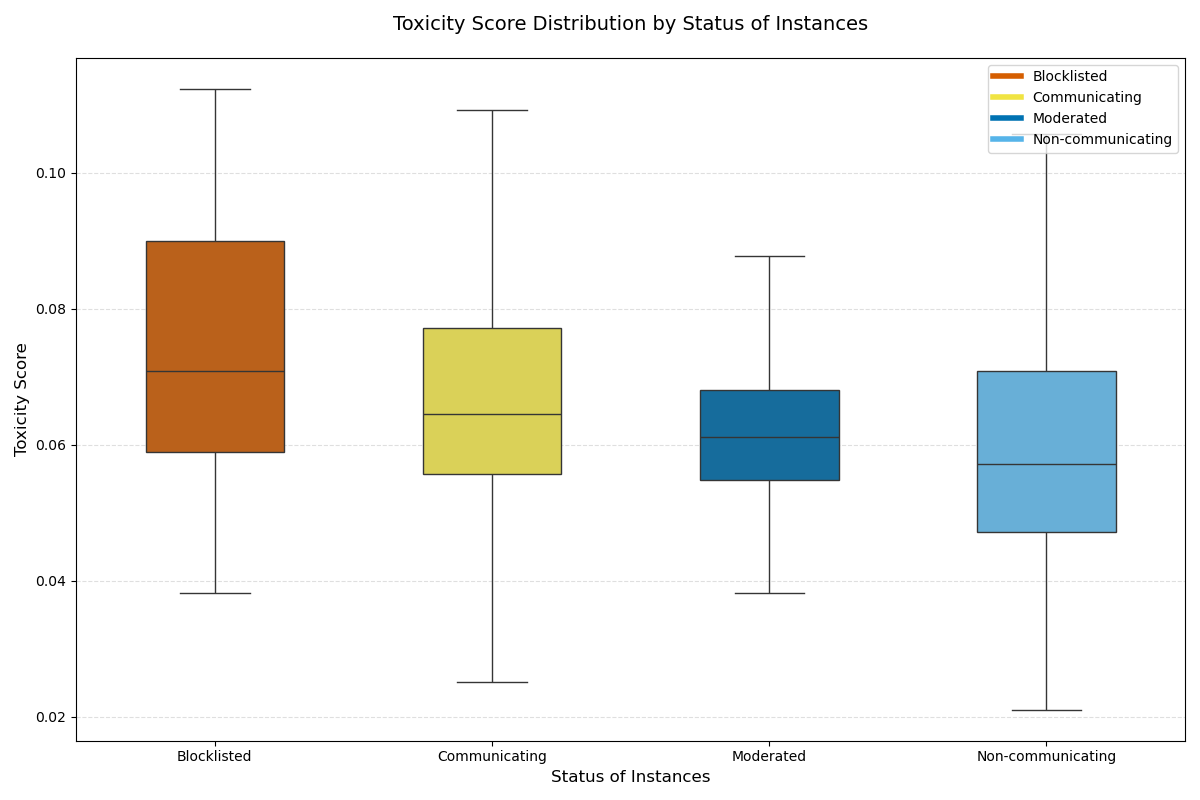
\includegraphics[width=\textwidth]{../material/blocklist_vs_covenant_boxplot.png}
    \caption{Comparison of average toxicity levels of instances across four instance categories: 
    \textbf{Moderated}: Mastodon Covenant members with active moderation policies;
    \textbf{Blocklisted}: Instances flagged for spreading inappropriate content; 
    \textbf{Communicating}: Instances interacting with blocklisted instances; 
    \textbf{Non-communicating}: Instances not interacting with any blocklisted instances.}
    \label{blocklisted-vs-covenant}
\end{figure}

But analyzing based on this classification presents a simplified perspective, as instances may be blocklisted for various reasons beyond toxicity, including spam or commercial content, rather than solely for inadequate moderation of hate speech. Nevertheless, the results in Figure~\ref{blocklisted-vs-covenant} offer initial evidence that moderation practices influence toxicity levels. The plot reveals the distribution of toxicity scores across four types of Mastodon instances, categorized by their moderation and communication behavior. Each boxplot summarizes the distribution of average toxicity scores per instance, as computed from the mean toxicity of all crawled toots. The plot reveals a distinct hierarchy in toxicity levels. 

\textbf{Blocklisted} instances demonstrate the highest toxicity levels, with a median score exceeding all other categories. The large interquartile range (IQR) reflects the small sample size in this group. Although those 13 instances can not be considered representative for all blocklisted instances, they show a clear trend of high toxicity.

\textbf{Moderated} instances following the mastodon covenant display lower toxicity levels overall. Their median toxicity is only slightly above that of non-communicating instances, and their IQR is narrower than the others. The compact boxplot indicates that the instances in this category are likely to be more homogenous in their moderation practices. This suggests that instances adhering to the Mastodon Covenant and actively moderating their content result in a less toxic environment.

Instances \textbf{communicating} with blocklisted as well as \textbf{Non-communicating} instances display a broad IQR and large whiskers distance. Therefore the results should be viewed with caution. Due to the imprecise grouping based on the communication with blocklisted instances, insances likely differ in terms of toxicity level. 

Nethertheless \textbf{communicating} instances show moderately elevated toxicity. While their median toxicity falls below blocklisted instances, it remains higher than the other categories. This supports the correlation between interaction with blocklisted instances being supposed to moderate poorly and increased toxicity. 

\textbf{Non-communicating} instances even display the lowest median toxicity. Although this might not be a perfect categorization, the overall trend confirms these instances maintain less toxic environments, likely due to their isolation from blocklisted content.

These findings support our hypothesis that moderation policies and federation behavior impact toxicity levels. Instances implementing active moderation or isolating from toxic environments show lower toxicity, while those interacting with blocklisted instances demonstrate increased toxic content. This hierarchy confirms that decentralized moderation practices directly influence platform climate.
